% TODO:


\documentclass[12pt, a4paper]{scrartcl}

\usepackage{graphicx}
\usepackage[ngerman]{babel}
\RequirePackage[ngerman=ngerman-x-latest]{hyphsubst}
\usepackage[utf8]{inputenc}
\usepackage[T1]{fontenc}
\usepackage[autostyle,german=guillemets]{csquotes}
\usepackage{verbatim}
\usepackage[singlespacing, onehalfspacing]{setspace}
\usepackage{lmodern}
\usepackage{pdfpages} % gut für Anhänge!
\usepackage{apacite}
\usepackage{url}
\usepackage{enumitem}
\usepackage{pdflscape}
%\usepackage{tabularx}
\usepackage{blindtext}
\usepackage{lipsum}
%\usepackage{relsize}
\usepackage{tocstyle}
\usepackage{color, colortbl}
%\usepackage[all]{nowidow}
\usepackage[pagewise]{lineno}
\usepackage{longtable}



\begin{document}

\title{Unterrichtsentwurf für eine Lehrprobe im Fach Sport}
\author{Dr. Hendrik Bunke}
\date{}
\thispagestyle{empty}

%\maketitle
\begin{center}
{
\includegraphics[height=1.1cm]{lis.png}}
\singlespacing
{\Huge{\textsf{\textbf{Unterrichtsentwurf für eine Lehrprobe im Fach Sport}}}}

\vspace{0.5cm}
\Large{Dr. Hendrik Bunke}



\end{center}



% !TEX root = 0.gesamt.tex



\singlespacing

\small
\begin{center}
\begin{tabular}{llllll}

\textbf{Schule:} & Datenschutz &
\textbf{Klasse:} & Datenschutz &
\textbf{Raum:} & Datenschutz \\
\textbf{Datum:}  & 01.04.2019  &
\textbf{Zeit:} & 08:30-09:30 Uhr &&\\


\\

\end{tabular}
%\begin{center}
\begin{tabular}{ll}
    \textbf{Thema der Unterrichtsstunde:} Passen in Bewegung\\
    \textbf{Thema der Unterrichtseinheit:} Fußball \\


\end{tabular}
\end{center}

\section*{Prüfungskommission}

\begin{tabular}{p{6cm} p{6cm}}
    \textbf{Vorsitzende:}& Datenschutz\\
    \textbf{Fachleiterin Sport:} & Datenschutz\\
    \textbf{Fachleiter Politik:} & Datenschutz\\
    \textbf{Fachleiterin BW:} & Datenschutz\\
    \textbf{Schulvertreterin:} & Datenschutz\\
    \textbf{Vertrauensreferendarin:} & Datenschutz\\

\end{tabular}





\normalsize


\footnotesize
\renewcommand{\contentsname}{Gliederung}
\usetocstyle{classic} %bewirkt, dass die Seitenzahlen genauso wie die Title formatiert sind (Größe!)
\tableofcontents

\newpage
\setcounter{page}{1}
%\onehalfspacing
\normalsize

% LIS Vorgabe ist 28-31 Zeilen pro Seite, weswegen das erheblich schönere
% \onehalfspacing von LaTeX nicht geht, damit wären's so rund 35. Keine Ahnung,
% ob das ein Problem wäre, aber sicher ist sicher
\setstretch{1,33}

%\linenumbers   % Zeilennummern um zu testen
%\modulolinenumbers[5]

% !TEX root = 0.gesamt.tex

\section{Lerngruppe und Unterrichtssituation}

\emph{aus Datenschutzgründen für die Veröffentlichung entfernt}


\subsection{Rahmenbedingungen}


\subsection{Kompetenzorientierte Lern- und Unterrichtsvoraussetzungen und erste Konsequenzen}


\subsection{Interaktionsbeziehungen}

% !TEX root = 0.gesamt.tex

% background color for special row in unterrichtssequenz
\definecolor{Gray}{gray}{0.9}

\section{Einordnung des Themas in curriculare Vorgaben und die Unterrichtssequenz}

Die Unterrichtseinheit \emph{Fußball} ordnet sich in das im Bildungsplan für
Gymnasien aufgeführte Bewegungsfeld \emph{Spielen} und den dort genannten
Sportbereich \emph{große Sportspiele} \cite[S.
10]{dersenatorfurbildungundwissenschaft2006a}. Im schulinternen Curriculum wird
als Unterrichtsvorhaben in den Klassen 5-6 für das Bewegungsfeld \emph{Spielen}
\enquote{Erste Einführung der Großen Spiele} gelistet \cite[S.
2]{kippenberg-gymnasiumbremen2011}. Als Kompetenzen werden in der vorliegenden
Stunde besonders gefördert \enquote{mit- und gegeneinander spielen},
\enquote{sich im Raum orientieren}, \enquote{partnerschaftlich agieren} sowie
\enquote{bisher erworbene allgemeine Spielfähigkeiten in das entsprechende
Spielgeschehen einbringen} \cite[S.
11]{dersenatorfurbildungundwissenschaft2006a}.

\subsection{Unterrichtssequenz}
\begin{scriptsize}
\begin{singlespacing}

\begin{longtable}{|p{3.5cm}|p{4.5cm}|p{7cm}|}
\hline
\textbf{Thema} & \textbf{Inhalt} & \textbf{didaktische Ziele / Kompetenzen}

\\
\hline
Der Ball ist dein Freund!
&
Ballgewöhnung und Dribbeln
&
Vorwissen Fußball aktivieren; Ballgewöhnung; Ball am Fuß führen; Wahrnehmung spezieller Fußballeigenschaften

\\
\hline
Den Ball zuspie"-len
&
Einführung Passen, Stoppen (statisch)
&
Innenspannstoß; korrekte Fußhaltung; präziser Pass zu Partner*in

\\
\hline
\rowcolor{Gray}
\textbf{Den Ball in Bewegung zuspielen}
&
\textbf{Passen in Bewegung}
&
\textbf{Anwendung Innenspannstoß in spielnaher Situation; Beobachtung und Beratung;}

\\
\hline

Tore schießen
&
Torschuss und Schusstechniken (Innenspann, Vollspann)
&
präzise schießen; kraftvoll und entschlossen schießen; schießen aus unterschiedlichen Spielsituationen

\\
\hline

Den Ball erobern
&
Zweikampf und Körpereinsatz
&
den Körper (fair) einsetzen; Körperkontakt; Körperhaltung; Ängste überwinden

\\
\hline

Zusammen spielen
&
Raumorientierung und Individualtaktik
&
Wahrnehmung von Raum und Mitspieler*innen; Positionierung im Raum; Freilaufen
\\
\hline

\end{longtable}
\end{singlespacing}
\end{scriptsize}



\vspace{0.5cm}

% !TEX root = 0.gesamt.tex
\section{Sachanalyse}

Fußball ist die weltweit beliebteste und am häufigsten betriebene Ballsportart
überhaupt. Die Gründe dafür sind vielfältig und reichen von der Einfachheit der
Regeln und des Spielgedankens über die Ritualisierung und gesellschaftliche
Verankerung bis hin zur sozialen Funktion \cite<vgl. dazu knapp
zusammenfassend>[S. 255f.]{stiehler1988}. Fußball gehört daher nach wie vor
auch fest in den Kanon schulischer Sportarten, schon weil
\enquote{Lebensweltbezug und Aktualität doch direkt gegeben} sind \enquote{und
nicht konstruiert werden} müssen \cite[S. 9]{lutgerodt2018}.

Das \emph{Passen} gehört neben dem Dribbeln und Schießen zu den drei
wesentlichen Grundtechniken des Fußballspiels. Betrachtet man die bis in den
Kinder- und Jugendbereich wirkende internationale Entwicklung des Fußballs in
den letzten zehn Jahren, hat das Passen als Grundelement des Ballbesitzfußballs
einen enormen Bedeutungszuwachs erfahren \cite<vgl.>[Kap. 2]{hyballa2014}. Und
auch wenn natürlich solche Anforderungen nicht in den Bereich von Kindern und
Jugendlichen übertragbar sind \cite[S. 226.f]{schomann2016}, kann das technisch
saubere Passen des Balls inzwischen als die wichtigste zu erlernende Technik
betrachtet werden, um im Fußball eine spezielle Spielfähigkeit zu
erlangen.\footnote{Dies spiegelt sich auch in den DFB-Schulungsmaterialien
wider, siehe z.B. \citeA[S. 29ff.]{kuhlmann2016}.}

Der \emph{Innenspannstoß} ist die am häufigsten angewandte Passtechnik und in
seiner statischen Form relativ einfach zu erlernen: Schussbein aufgedreht, Ball
mit dem Zentrum der Innenseite treffen, Standbein steht neben Ball;
\cite{schomann2016}. Die Anforderungen werden jedoch komplexer, wenn in
Bewegung gepasst wird. Hier kommt die Abstimmung mit dem Passempfänger hinzu,
Laufwege müssen antizipiert werden und die Passausführung wie auch die
Ballannahme müssen mit der eigenen Laufbewegung koordiniert werden.

% !TEX root = 0.gesamt.tex
\section{Didaktische Analyse}

\textbf{Didaktische Leitidee:} Die SuS kombinieren das in der letzten Stunde
erlernte bzw. verfestigte statische Passen mit Laufbewegungen auf engem Raum.
Dabei wird die Komplexität durch das Abstimmen mit der Partnerin / dem Partner
sowie dem Ausweichen weiterer übender Pärchen erhöht und die Bewältigung durch
kriterienorientierte kognitive Reflexion mit \enquote{Personal Coaches} und in
der Lerngruppe unterstützt. Übungsanreiz bietet ein Wettbewerb, in dem die SuS
in begrenzter Zeit möglichst viele Pässe durch vorgegebene Ziele spielen
sollen.

Nimmt man die Grundfragen der didaktischen Analyse nach \citeA{klafki1962} zum
Maßstab, ist zunächst die hohe \textbf{Gegenwartsbedeutung} des Themas Fußball
hervorzuheben. Fußball als gesellschaftlich, kulturell und sozial tief
verankerte Sportart bietet hohes soziales Integrations- und
Interaktionspotenzial. Sie auf auch nur einem Basis-Niveau zu verstehen und
beherrschen, befähigt zu gesellschaftlicher und sozialer Teilhabe. Dies gilt
für alle SuS, ganz besonders jedoch -- bezogen auf die Lerngruppe der
vorliegenden Stunde -- für die Mädchen. Während eine Fußballsozialisation für
Jungen weitgehend selbstverständlich, zumindest aber leicht zugänglich ist,
haben Mädchen es diesbezüglich aus verschiedenen Gründen immer noch erheblich
schwerer. Speziell für sie besteht die \textbf{Zukunftsbedeutung} des Themas
deshalb auch darin, die Chancen und Möglichkeiten, die der Fußball bietet, für
sich genauso nutzen zu können, wie Jungen das können. Man kann in Anlehnung an
einen Begriff aus der Sozialpsychologie von \enquote{Empowerment} sprechen, was
u.a. auch das Erwerben von Kompetenzen zur gesellschaftlichen und kulturellen
Teilhabe umfasst. \enquote{Bezogen auf Mädchenfußball heißt das, dass Mädchen
dazu ermuntert werden sollen in bisher männerdominierte Welten einzudringen und
sich dort zu behaupten} \cite[S. 13]{kugelmann2009}. In naher Zukunft ist in
diesem Kontext für die UE auch die vom 7.6.-7.7.2019 in Frankreich
stattfindende Fußball-Weltmeisterschaft der Frauen bedeutsam, die den
Schülerinnen im Anschluss an die Unterrichtseinheit unmittelbar
Identifikations- und Anwendungsmöglichkeiten bietet.

Das Thema \emph{Passen} als Schwerpunkt der vorliegenden wie auch der
vorhergehenden Stunde ist prinzipiell nicht nur für Fußball, sondern für nahezu
alle Ballsportarten von grundlegender Bedeutung. So kann denn auch die in
dieser Stunde schwerpunktmäßig durchgeführte Übung hinsichtlich der Laufwege,
der Raumorientierung, dem Bewegen mit Ball und beim Passen nahezu 1:1 auf
andere Sportspiele übertragen werden (\textbf{exemplarische Bedeutung}).
\textbf{Zugänglich} wird den SuS das Passen in Bewegung zunächst durch die
Bewusstmachung, dass in realen Spielsituationen so gut wie nie nur im Stand
gepasst wird und -- aufgrund von Gegnereinwirkungen -- auch nicht werden kann.
Darauf aufbauend wird auch das Thema Geschwindigkeit (Gegner überlaufen,
überpassen) angesprochen. Motivational unterstützt wird dies durch den
Wettbewerb (\emph{wer schafft die meisten Tore in 2 Minuten zu durchspielen?}).
Geschwindigkeit stellt auch die erste Ebene der \textbf{inhaltlichen
Strukturierung} dar. Weitere sind Pass-Präzision sowie die Koordination (Raum)
und Absprache mit der/dem Mitspieler*in.

% !TEX root = 0.gesamt.tex
\section{Kompetenzen}


\scriptsize
\singlespacing

\begin{longtable}{|p{3cm}|p{4cm}|p{4cm}|p{4cm}|}

\hline
\textbf{Kompetenz Dimension} &

\textbf{Standards der Bildungspläne \newline \newline die Schüler*innen können...} &

\textbf{Aufgabenstruktur (Performanz) \newline \newline ...indem sie...} &

\textbf{Differenzierte, auf die Lern"-gruppe be"-zo"-gene For"-mulierung des Kompetenzniveaus}

\\
\hline

\textbf{Fachkompetenz}
&
...mit- und gegeneinander spielen, \newline
...sich im Raum orientieren, \newline
...partnerschaftlich agieren, \newline
...bisher erworbene allgemeine Spielfähigkeiten in das entsprechende Spielgeschehen einbringen
&
...zu zweit versuchen, in begrenzter Zeit eine möglichst hohe Anzahl von Markierungen zu durchpassen \newline
...in einem eng begrenztem Spielfeld die eigene Stellung im Raum, die des Partners, des Balles und der Pass-Ziele wahrnehmen und in adäquate Bewegungen im Raum umsetzen \newline
...sich absprechen
&
- nur mit starkem Fuß passen\newline
- beidfüßig oder mit Außenspann passen \newline

\\
\hline

\textbf{Methodenkompetenz} &
...den Trainingsprozess mitgestalten und kleinere Aufgaben übernehmen
&
...als \emph{Personal Coaches} andere Spieler*innen kriteriengeleitet beobachten und beraten
&

\\
\hline

\textbf{Sozialkompetenz} &
 ...kooperieren \newline
 ...anderen helfen und und Hilfe annehmen
&
...zu zweit versuchen, in begrenzter Zeit eine möglichst hohe Anzahl von Markierungen zu durchpassen \newline
...beraten und sich beraten lassen
&
- ohne verbale Absprachen gemeinsame Wege finden \newline
- einen bestimmten Weg vorab vereinbaren (im Uhrzeigersinn o.ä.)
\\
\hline

\textbf{Personalkompetenz} &
...Leistungsbereitschaft zeigen \newline
...teamfähig sein
&
...sie eine möglichst hohe Anzahl von Markierungen durchpassen \newline
...mit Kritik durch die \enqoute{Personal Coaches} sachlich umgehen können

&



\\
\hline

\textbf{Sprachkompetenz} &
...angemessen Fachbegriffe benutzen \newline
...Bewegungen und Beobachtungen korrekt und verständlich beschreiben
&
...die grundlegende Passtechnik \emph{Innenspannstoß} benennen können \newline
...die wesentlichen Merkmale des Innenspannstoßes verständlich beschreiben

&

\\
\hline

\end{longtable}


\normalsize
\onehalfspacing

% !TEX root = 0.gesamt.tex
\section{Methodische Überlegungen}

Methodisch im Zentrum der Stunde steht eine einzige Übung, das Passen mit
einem/einer Partner*in durch einen mit Floormarkern\footnote{Es werden hier
keine sonst üblichen Pylonen oder einfache Hütchen verwendet, da diese auf
Hallenboden speziell bei Fußballübungen leicht verrutschen oder umfallen.
Floormarker sind auch auf Hallenboden rutschfest und gleichzeitig gut
sichtbar.} markierten \enquote{Wald} oder Parcours. Die Konzentration auf eine
Übung ermöglicht zum einen motorische und kognitive Vertiefung, zum anderen
kann durch die Beibehaltung eines sehr einfachen Aufbaus Zeit für die
Erarbeitung gewonnen werden. Zweiter methodischer Kern-Aspekt ist, in Anlehnung
an das Konzept des \enquote{Personal Coaching} \cite{flemming2009}, die
einfache  kriteriengestützte Beobachtung und Beratung der SuS untereinander.
Dies ermöglicht zum einen eine angesichts der geringen Größe der Halle
notwendige organisatorische Teilung der Lerngruppe, ohne dass eine Gruppe
passiv nur zuschauen muss \cite<vgl.>[S. 13]{wagener2018}. Zum anderen fördert
es zusätzlich zur technischen Fachkompetenz \enquote{kooperatives Verhalten}
und \enquote{methodisches Denken} \cite[S. 20]{flemming2009}.

Nach der Begrüßung der SuS im ritualisiert eingeführten \enquote{Klassenzimmer}
werden zunächst zur \textbf{Aktivierung des Vorwissens} die in der letzten
Stunde erarbeiteten wesentlichen Merkmale des Innenspannstoßes wiederholt und
an der Tafel notiert. Sie sind auch Bestandteil der Beobachtungsaufgaben im
Hauptteil. Nachfolgend teilt die Lehrkraft mittels
\emph{TeamShake}\footnote{\emph{TeamShake} ist eine App, mit der sich leicht
Guppen für Sportspiele einteilen lassen. Dabei geschieht die Einteilung nicht
nur zufallsbasiert, sondern kann nach Stärken, Geschlecht etc. konfiguriert
werden.} die Partner für das folgende Aufwärmspiel zusammen. Die Paarungen
bleiben für den Rest der Stunde bestehen und werden im Hauptteil zu 4-er
Gruppen zusammengesetzt.

Das folgende Spiel dient der allgemeinen und speziellen \textbf{Erwärmung},
aber auch der Wiederholung des in der letzten Stunde erlernten statischen
Passens und der Partnergewöhnung.\footnote{Ein Paar agiert als Fängergruppe,
die anderen laufen jeweils Hand in Hand durch die Halle. Ein Paar, das getickt
wurde, macht auf dem Boden zwei Brücken hintereinander. Durch dieses
\enquote{Tor} muss der Ball von einem anderen Paar einmal durchgepasst werden,
um die Gefangenen zu befreien.}

Der Einstieg in die \textbf{Erarbeitungsphase} beginnt mit einer Frage der
Lehrkraft, mit der das bisher Gelernte mit den Vorstellungen der SuS vom
\enquote{richtigen} Fußballspielen abgeglichen werden. Die SuS erkennen
\enquote{Bewegung} als wesentlichen Unterschied. Ausgehend davon erfolgt die
Erläuterung von Ablauf und Zweck der folgenden Übung. Zur visuellen
Unterstützung werden Parcours, Lauf- und Passwege auf der Tafel skizziert. Der
Zusammenschluss der Paare zu Vierergruppen erfolgt durch die SuS, da für die
Bewertungsaufgaben ein gewisses Vertrauensverhältnis nötig ist
\cite<vgl.>{flemming2009}. Im ersten Durchgang der Übungsphase durchläuft jedes
Paar einmal für zwei Minuten den Parcours und wird dabei beobachtet von dem
zweiten Paar der 4er-Gruppe, den \emph{Coaches}. Hier liegt der Schwerpunkt
zunächst auf der Gewöhnung, die SuS sollen vor allem auf die Umsetzung der
erlernten Passtechnik sowie die enge Ballführung achten. Den Gruppen wird nach
jedem Durchgang kurz Gelegenheit zur Besprechung gegeben. In einem folgenden
zweiten Durchgang sollen dann die durchpassten Tore gezählt werden, um zum
einen einen Ansporn zu bieten und um zum anderen später Vergleichsmöglichkeiten
zu haben. Diese Aufgabe übernehmen die Coaches. Auch hier wird wieder kurz
Gelegenheit zum Besprechen gegeben. In einer gemeinsamen
\textbf{Zwischenbesprechung} wird zum einen reflektiert (\emph{was ist euch
aufgefallen?}), zum anderen werden Kriterien gesammelt, die die Bewältigung des
Parcours sicherer und schneller machen können (in Bewegung bleiben, präziser
passen, mehr passen). Diese Kriterien finden sich auch in den Bewertungsbögen
für die Coaches wieder, von denen jedes Paar (inkl. Klemmbrett und
Kugelschreiber) nun einen erhält. In zweiten Teil der Erarbeitung wird nun das
Durchlaufen des Parcours von den Coaches mit Hilfe der genannten Kriterien
bewertet, auf den Bögen notiert und anschließend mit der \enquote{Mannschaft}
besprochen. Letztere durchläuft dann mit den Tipps der Coaches noch einmal den
\enquote{Wald}. Nach einer weiteren kurzen Besprechungsphase zwischen Coaches
und Mannschaften erfolgt der Wechsel. Zur \textbf{Differenzierung} kann in
dieser Phase besonders leistungsstarken SuS der Auftrag gegeben werden,
beidfüßig zu passen (abwechselnd links/rechts) oder auch dein Außenspannpass zu
probieren. SuS mit Problemen beim Passen kann ein Punktebonus gegeben werden
und sie werden angehalten, statt auf Tempo vor allem auf Präzision und
Absprache zu achten. In der abschließenden \textbf{Auswertung und Sicherung}
nach dem Abbau des Parcours fragt die Lehrkraft zunächst nach den maximal
durchspielten Toren (\textbf{Wettbewerb}) und fragt dann die SuS, was von den
genannten Kriterien gut klappt und wo noch geübt werden sollte. Die Ergebnisse
werden an der Tafel gesichert. Daneben werden die Bewertungsbögen (die anonym
bleiben) eingesammelt und später von mir ausgewertet.

Als \textbf{didaktische Reserve} kann mit demselben Aufbau auf zwei Feldern ein
Blitzturnier mit den bereits eingeteilten 4er-Gruppen gespielt werden. Ziel ist
das Durchpassen eines der Floormarker-Tore, bei einem Treffer werden die
Mannschaften gewechselt.

% !TEX root = 0.gesamt.tex

% \newcolumntype{L}[1]{>{\raggedright\arraybackslash}p{#1}} % linksbündig mit Breitenangabe

\begin{landscape}
%\thispagestyle{empty}
\section{Verlaufsplan}

\singlespacing
\scriptsize
\begin{longtable}{p{2cm}|p{5.5cm}|p{5.5cm}|p{2cm}|p{2cm}|p{4cm}}

\textbf{Phase} &
\textbf{Aktivität Lehrkraft} &
\textbf{Aktivität SuS} &
\textbf{Sozialform} &
\textbf{Medien, Material} &
\textbf{didaktisch-methodischer Kommentar}
\\
\hline
\textbf{Einstieg}
&
- begrüßt SuS und Gäste \newline
- bittet SuS um Zusammenfassung der letzten Stunde und notiert die genannten Kriterien an Tafel \newline
- nennt das heutige Thema, verweist auf die notierte Tagesordnung \newline
- teilt die Paare ein \newline
- erläutert das Aufwärmspiel \newline
&
- begrüßen L und Gäste \newline
- nennen wesentliche Inhalte der letzten Stunde \newline
- wiederholen Kriterien des \emph{Innenspannstoßes}\newline
&
Plenum / UG
&
Tafel, Kreide/Stift, Smartphone, TeamShake
&
jede Stunde startet im Klassenzimmer, strukturierter Beginn

\\
\hline
\textbf{Aufwärmen}
&
bestimmt neue Fänger-Pärchen (ggf. auch zwei)
&
spielen
&
Spiel, PA
&
2-3 Bälle
&
Erwärmung dient auch der Wiederholung (statisches Passen) und der Vorbereitung auf den Hauptteil (PA)
\\
\hline

\textbf{Erarbeitung I}
&
- \emph{Was fehlt noch zum \enquote{richtigen} Passen?} \newline
- erläutert die Aufgabe, skizziert Aufbau und mögliche Pass- und Laufwege, demonstriert ggf. einmal mit eine*r Schüler*in die Aufgabe \newline
- beaufsichtigt, gibt Hinweise und Start-/Stopp Signale
&
- nennen \emph{Bewegung} als fehlendes Element \newline
- finden sich in 4er-Gruppen zusammen \newline
- jedes Paar durchläuft zweimal für 2 Minuten den \enquote{Wald}, das jeweils andere Paar beobachtet und gibt Hinweise auf Basis der Kriterien und zählt die durchpassten Tore (im 2. Durchgang)
&
Plenum / UG, PA, GA
&
Tafel, Floormarker, 7-8 Fußbälle
&

\\
\hline
\textbf{Zwischen"-be"-sprechung}
&
- lobt die SuS und fragt nach Schwierigkeiten \newline
- \emph{Was könnte man machen, um schneller und sicherer durch den Wald zu kommen?} \newline
-  stellt den Beobachtungsbogen vor \newline
&
nennen: in Bewegung bleiben (so wenig wie möglich stehen), präziser passen, mehr passen
&
Plenum
&
Beobach"-tungs"-bogen
&
\\
\hline
\textbf{Erarbeitung II} \newline
&
unterstützt die Coaches und die Beratung der Spieler*innen
&
- laufen mindestens 2x den Parcours  \newline
- Coaches beobachten, zählen, notieren, beraten
&
PA, GA
&
Floormarker, Beobachtungsbögen, Klemmbretter, Kugelschreiber, 7-8 Fußbälle
&
- die Coaches wechseln nach dem ersten Durchgang die Aufgaben (Zählen, Notieren/Beobachten) \newline
- Differenzierung: beidfüßig, langsamer

\\
\hline
\textbf{Abschluss}
&
- Ergebnisvergleich: wer hat die meisten Tore geschafft? \newline
- Was von den genannten Kriterien ging schon gut, was wollen wir noch üben? \newline
- Wie war das Arbeiten mit den Coaches? \newline
- bedankt sich und verabschiedet die SuS
&
- nennen Ergebnisse \newline
- benennen noch einmal die Kriterien und bewerten das bisher Erlernte sowie die Methode der \emph{Personal Coaches} \newline
- geben Stimmungsbild per Daumenprobe
&
Plenum (Klassenzimmer)
&
Tafel, Stift oder Kreide
&

\end{longtable}
\end{landscape}

\normalsize



% \newpage
\clearpage
\pagestyle{empty}
\singlespacing
\bibliography{zotero.bib}
\bibliographystyle{apacite}

\newpage
\section*{Erklärung}
Diese schriftliche Planung habe ich selbstständig angefertigt. Andere als die
angegebenen Hilfsmittel habe ich nicht benutzt. Die Stellen der schriftlichen
Ausarbeitung, die anderen Werken, auch eigenen oder fremden unveröffentlichten
Prüfungsarbeiten, im Wortlaut oder ihrem wesentlichem Inhalt nach entnommen
sind, habe ich mit genauer Angabe der Quelle kenntlich gemacht.

\vspace{1cm}Bremen, 29.03.2019

\vspace{3cm}(Dr. Hendrik Bunke)



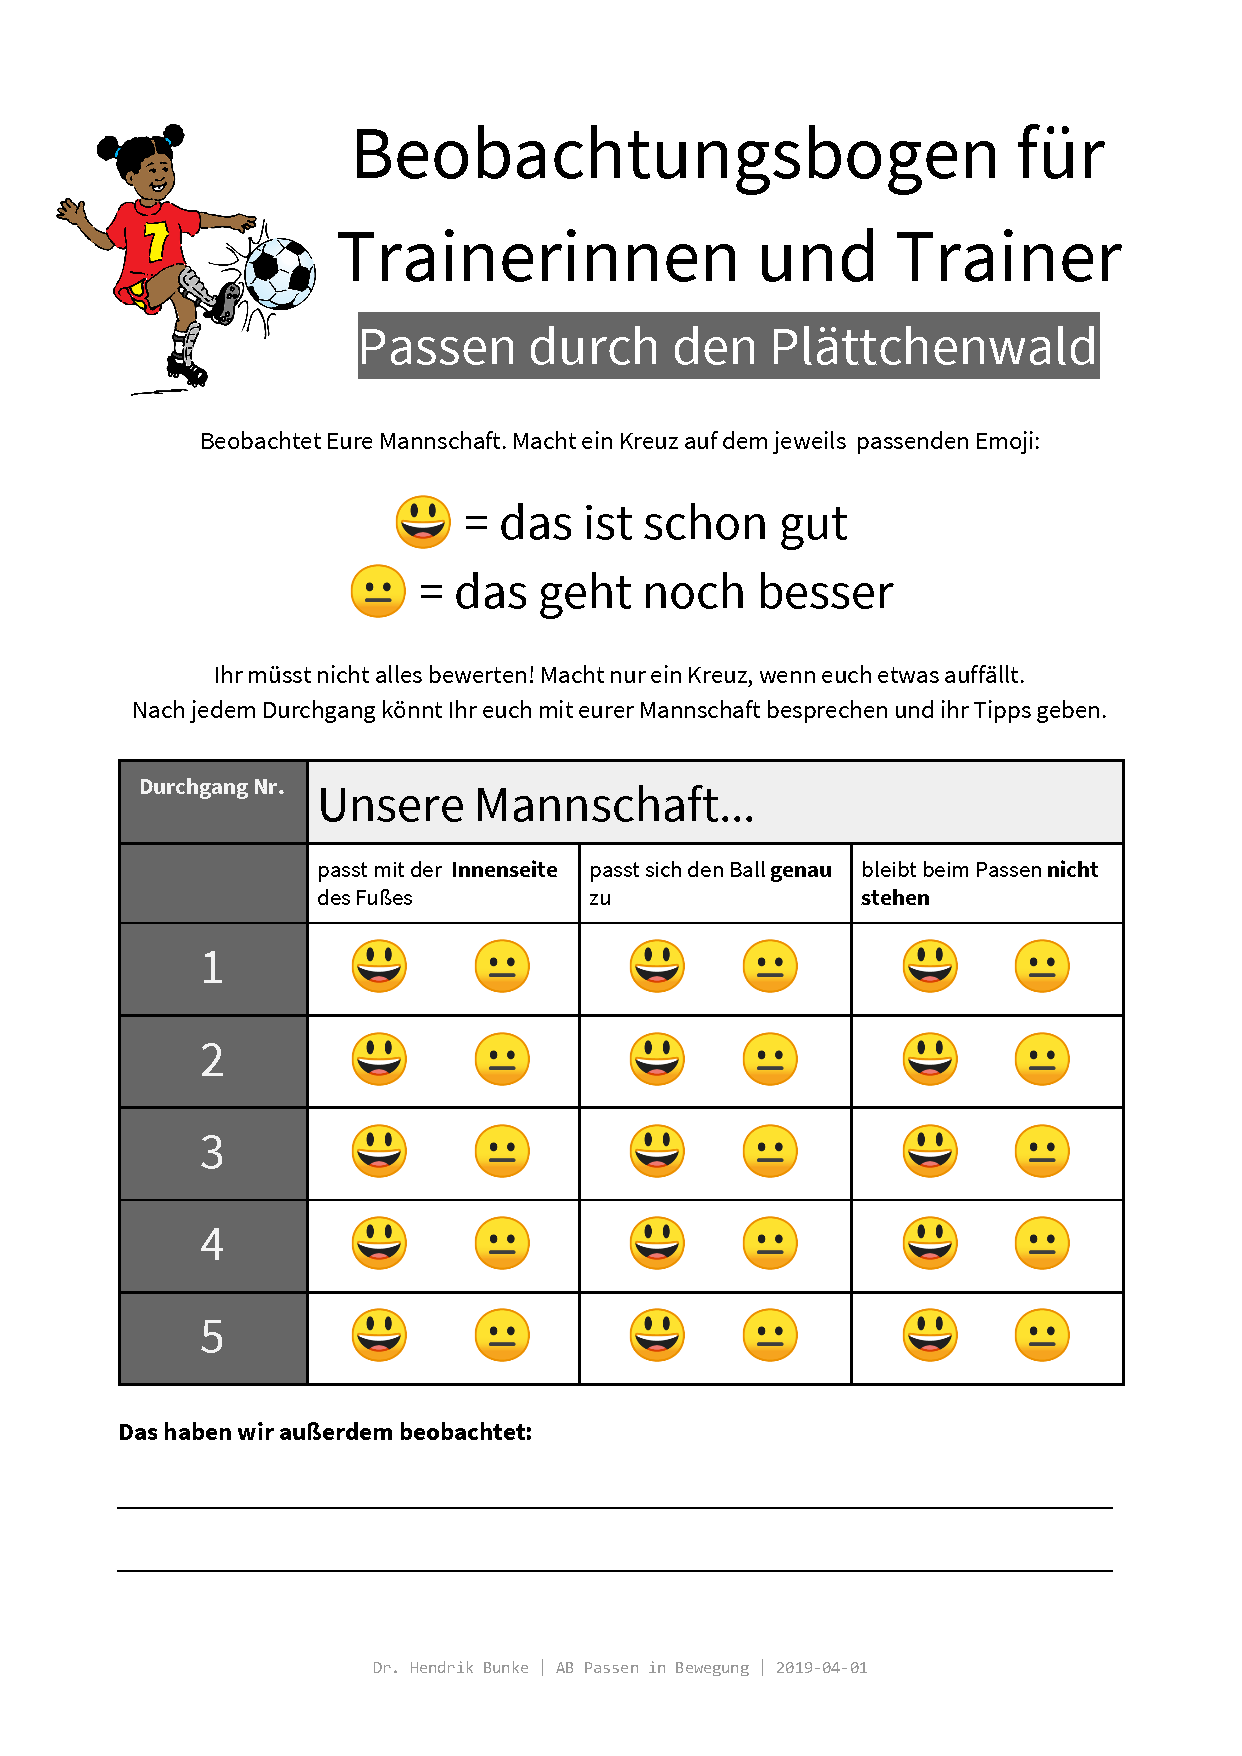
\includepdf[pages=-]{beobachtungsbogen.pdf}


\end{document}
